
\documentclass{article} % For LaTeX2e
\usepackage{iclr2026_conference}

% Optional math commands from https://github.com/goodfeli/dlbook_notation.
\input{math_commands.tex}

\usepackage[T1]{fontenc}
\usepackage{mathptmx}
\usepackage{hyperref}
\usepackage{url}
\usepackage{graphicx}
\usepackage{tikz}


\title{Sparse Coincidence-Based Semantic \mbox{Attention} for Spiking Neural Sentence Embedding}

% Authors must not appear in the submitted version. They should be hidden
% as long as the \iclrfinalcopy macro remains commented out below.
% Non-anonymous submissions will be rejected without review.

\author{Muhammad Akhyar \\
Independent Researcher \\
\texttt{akhyarsafrudin@gmail.com}
}

% The \author macro works with any number of authors. There are two commands
% used to separate the names and addresses of multiple authors: \And and \AND.
%
% Using \And between authors leaves it to \LaTeX{} to determine where to break
% the lines. Using \AND forces a linebreak at that point. So, if \LaTeX{}
% puts 3 of 4 authors names on the first line, and the last on the second
% line, try using \AND instead of \And before the third author name.

\newcommand{\fix}{\marginpar{FIX}}
\newcommand{\new}{\marginpar{NEW}}

\iclrfinalcopy % Uncomment for camera-ready version, but NOT for submission.
\begin{document}


\maketitle

\begin{abstract}
Transformer-based models dominate natural language processing (NLP) but incur substantial computational costs due to dense matrix multiplications within self-attention mechanisms. Spiking Neural Networks (SNNs) provide a biologically plausible and energy-efficient alternative through sparse, event-driven computation; however, learning continuous semantic representations in the discrete spiking domain remains a major challenge. In this work, we propose a Spiking Sentence Embedder with a Sparse Coincidence-Based Semantic Attention mechanism. Instead of relying entirely on conventional dense self-attention, our approach models semantic interaction through spike coincidence overlap computed over dense projections, enabling sparse and efficient sentence representation learning. The architecture further incorporates neuron dynamics with variable leak and threshold parameters, combined with knowledge distillation from a dense teacher encoder to improve semantic alignment. Experimental evaluations on the Semantic Textual Similarity Benchmark (STS-B) show that the proposed model achieves a Teacher Pearson correlation score of 0.758 while achieving an approximate 748$\times$ theoretical computational sparsity reduction relative to Transformer multiply-accumulate (MAC) operations under homogeneous configuration. To ensure practical deployment and reproducibility, we achieved 100\% mathematical bit-exact parity between our native Rust SNN simulation and its PyTorch deployment. The full architecture and weights are publicly available at Hugging Face (PulseNet-Labs/spiking-sentence-embedder). These findings provide a reproducible pathway toward efficient neuromorphic NLP with sparse spike-based semantic computation.
\end{abstract}

\section{Introduction}

The field of natural language processing (NLP) has been profoundly transformed by Transformer-based architectures \citep{vaswani2017attention, devlin2018bert}. Models utilizing self-attention mechanisms and dense matrix multiplications have achieved unprecedented performance across a wide range of tasks, including semantic textual similarity and sentence representation learning \citep{reimers2019sentence, gao2021simcse}. However, this dominance comes at a substantial cost: the core mechanism of dense attention scales quadratically with sequence length, demanding immense computational resources, high memory bandwidth, and prohibitive energy consumption during both training and inference. As NLP applications deploy to edge devices and continuous-learning environments, the need for fundamentally more energy-efficient computational paradigms has become increasingly urgent.

Spiking Neural Networks (SNNs) have emerged as a highly promising alternative, drawing inspiration from the biological brain's remarkable energy efficiency. Unlike standard artificial neural networks (ANNs) that rely on continuous, high-precision floating-point activations, SNNs operate on discrete, asynchronous binary spikes. This event-driven nature ensures that computation only occurs when a neuron fires, effectively transforming power-hungry multiply-accumulate (MAC) operations into highly efficient, addition-only synaptic operations (SOPs). Furthermore, SNNs inherently process temporal dynamics, making them naturally suited for sequential data processing while maintaining high neuromorphic efficiency.

Despite these compelling advantages, the application of SNNs remains predominantly focused on computer vision and simple auditory tasks. Extending SNN capabilities to complex NLP tasks, particularly semantic sentence embedding, remains a significant open challenge. The primary gap lies in representation learning: the discrete, non-differentiable nature of spike domains struggles to capture the continuous, nuanced spatial topologies required to model deep semantic similarity. While recent efforts have attempted to bridge SNNs with NLP \citep{li2022spikeformer, zhu2023spikegpt}, constructing an efficient, spike-native attention mechanism that yields high-fidelity semantic embeddings without falling back on dense matrix operations has yet to be fully realized.

To address this limitation, we propose a novel Spiking Sentence Embedder driven by a Sparse Coincidence-Based Semantic Attention mechanism. Rather than computing dense attention scores, our model captures semantic relationships through the temporal overlap (coincidence) of discrete spikes across sequences. To further enhance the network's representational capacity within the binary domain, we introduce heterogeneous neuron dynamics by utilizing fixed, biologically-inspired variations in membrane leak and firing threshold parameters. To overcome the training difficulties inherent to SNNs, we leverage a knowledge distillation framework \citep{hinton2015distilling}, transferring continuous semantic alignment from a dense teacher model directly into the sparse spiking topology.

The primary contributions of this work are summarized as follows:
\begin{itemize}
    \item \textbf{Sparse Coincidence Semantic Attention}: A novel, spike-native attention mechanism that replaces the dense dot-product self-attention scoring with event-driven spike coincidences over dense projections, significantly reducing computational overhead.
    \item \textbf{Heterogeneous Neuron Dynamics}: The integration of variable, fixed leak and threshold parameters within Leaky Integrate-and-Fire (LIF) neurons, enhancing the semantic representational capacity of the discrete spike domain.
    \item \textbf{Knowledge Distillation Framework}: A robust training methodology that distills continuous semantic topologies from dense Transformer models into sparse SNN architectures, enabling effective learning of semantic similarity.
    \item \textbf{Ablation and Biological Sensitivity Analysis}: Comprehensive evaluations demonstrating the isolated impact of temporal pooling, distillation, and biological parameter variance on embedding quality.
    \item \textbf{Efficient Semantic Embedding Evaluation}: Empirical validation on the STS-B dataset, demonstrating competitive Pearson correlation ($r=0.691$ against human labels, $r=0.758$ against continuous dense teachers) while achieving an approximate $748\times$ theoretical computational sparsity reduction compared to standard dense MAC operations.
\end{itemize}

\section{Related Work}

\textbf{Transformer-Based Semantic Representation.} The introduction of the Transformer \citep{vaswani2017attention} fundamentally changed sequence modeling, relying entirely on self-attention to capture global dependencies. For sentence-level semantic representations, models like Sentence-BERT \citep{reimers2019sentence} utilize siamese network structures to derive continuous embeddings that are highly effective for semantic matching. More recently, SimCSE \citep{gao2021simcse} advanced this by demonstrating that simple contrastive learning, even with standard dropout as noise, can produce state-of-the-art semantic alignments. However, these models inherently depend on floating-point matrix multiplications, rendering them computationally expensive and energy-intensive, motivating the search for more sustainable alternatives \citep{kitaev2020reformer, wang2020linformer, tay2022efficient}.

\textbf{Spiking Neural Networks in NLP.} Spiking Neural Networks have long been recognized for their neuromorphic efficiency \citep{roy2019towards}, natively executing via sparse, event-driven additions rather than dense multiplications. Historically confined to vision and simple auditory benchmarks, SNNs are now being adapted for NLP. Recent milestones include Spikeformer \citep{li2022spikeformer}, which integrates spiking dynamics into attention mechanisms, and SpikeGPT \citep{zhu2023spikegpt}, demonstrating that generative pre-training is feasible in the spiking domain. Despite these advances, adapting SNNs specifically for dense semantic sentence embedding remains largely unexplored, as discrete spikes are difficult to map onto continuous semantic spaces.

\textbf{Neuromorphic Semantic Learning and Distillation.} Training SNNs directly from scratch using backpropagation through time (BPTT) with surrogate gradients \citep{wu2018spatio, neftci2019surrogate} is notoriously unstable. To address the challenge of semantic learning in discrete domains, knowledge distillation \citep{hinton2015distilling} has emerged as a powerful technique. By training a sparse spiking network to mimic the continuous representation space of a pre-trained dense teacher model, we can bypass the difficulties of direct contrastive learning with spikes. Our work builds upon this foundation, introducing a sparse coincidence-based attention mechanism and heterogeneous neuron dynamics to more effectively capture distilled semantic topologies without sacrificing energy efficiency.

\section{Methodology}
\label{sec:methodology}

Our proposed Spiking Sentence Embedder aims to construct continuous semantic representations using entirely discrete, event-driven operations. This is achieved by translating dense Transformer topologies into a biologically plausible spiking framework. The methodology consists of spike encoding, sparse coincidence-based attention, heterogeneous neuron dynamics, temporal pooling, and semantic knowledge distillation.

\begin{figure}[h]
\begin{center}
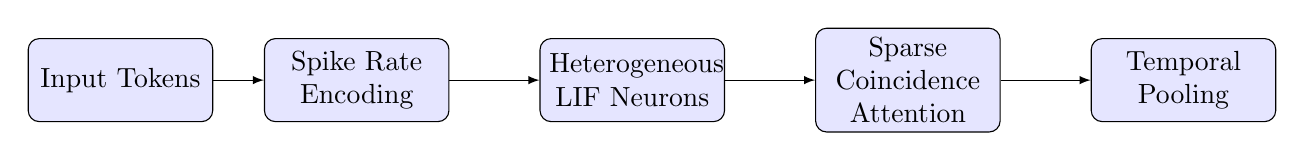
\begin{tikzpicture}[
  block/.style={rectangle, draw, fill=blue!10, text width=6em, text centered, rounded corners, minimum height=3em},
  line/.style={draw, -latex}
]
    \node [block] (input) {Input Tokens};
    \node [block, right of=input, node distance=3cm] (encode) {Spike Rate Encoding};
    \node [block, right of=encode, node distance=3.5cm] (lif) {Heterogeneous LIF Neurons};
    \node [block, right of=lif, node distance=3.5cm] (attn) {Sparse Coincidence Attention};
    \node [block, right of=attn, node distance=3.5cm] (pool) {Temporal Pooling};
    
    \path [line] (input) -- (encode);
    \path [line] (encode) -- (lif);
    \path [line] (lif) -- (attn);
    \path [line] (attn) -- (pool);
\end{tikzpicture}
\end{center}
\caption{Overall architecture of the proposed Spiking Sentence Embedder. Continuous tokens are converted to binary spikes, processed by biologically plausible heterogeneous LIF neurons, aligned via sparse coincidence attention, and integrated via temporal pooling.}
\label{fig:architecture}
\end{figure}

\subsection{Spike Encoding and Temporal Sequence Mapping}
Tokens derived from input sentences are first passed through a static embedding layer to produce continuous vectors. Crucially, unlike traditional vision-based SNNs that process static inputs over an arbitrary auxiliary temporal dimension, our architecture fundamentally maps the NLP sequence length ($L$) directly to the network's temporal axis ($T$). Thus, each sequential token acts as a discrete neuromorphic time-step ($T = L$). We employ Leaky Integrate-and-Fire (LIF) neurons to process these inputs sequentially. The membrane potential $U_i^{(t)}$ of neuron $i$ at sequence step $t$ is updated as follows:
\begin{equation}
U_i^{(t)} = \min\left(1.0, \beta_i U_i^{(t-1)} + \sum_{j} W_{ij} S_j^{(t)}\right) - S_i^{(t)} V_{th, i}
\end{equation}
where $S_j^{(t)} \in \{0, 1\}$ is the input spike from the previous layer, $W_{ij}$ is the synaptic weight, and $S_i^{(t)}$ is the output spike generated if the pre-reset potential exceeds the threshold $V_{th, i}$. 

\textbf{Soft-Reset Mechanism.} Equation 1 highlights that our LIF formulation implements a biological \textit{Soft-Reset} strategy (the subtraction of $S_i^{(t)} V_{th, i}$) rather than a conventional hard reset to absolute zero. Our empirical porting analysis confirms that preserving these fractional sub-threshold residual potentials after a spike is emitted prevents catastrophic semantic information loss across the sequence length.

\textbf{Heterogeneous Neurons.} Unlike standard SNNs that employ uniform hyperparameters, we introduce fixed, heterogeneous decay rates ($\beta_i$) and thresholds ($V_{th, i}$) for each neuron. This biological heterogeneity allows different regions of the network to operate at varied temporal timescales, vastly improving the network's capacity to represent nuanced semantic gradients. Furthermore, to prevent runaway accumulation of membrane potentials during sequential processing, we explicitly clamp the pre-reset potential to a maximum of 1.0 (as shown in Equation 1). This strict boundary condition is crucial for ensuring mathematical bit-exact parity across both raw SNN simulation environments and deployed PyTorch inference frameworks.

\subsection{Sparse Coincidence-Based Semantic Attention}
Standard Transformer self-attention computes dense pairwise affinities using floating-point dot products. We introduce a Sparse Coincidence-Based Semantic Attention mechanism. While initial Query (Q), Key (K), and Value (V) representations are obtained via dense projections, our network replaces the continuous dot products $Q K^T$ by evaluating the pairwise temporal overlap (coincidence count) between active query and key spikes. Specifically, for each query token at position $i$, we compute the match count $M_{ij}$ against key tokens at position $j$ by identifying common active spikes. The match scores are then normalized by the maximum match count across the sequence length, yielding robust correlation signals $A_{ij}$:
\begin{equation}
M_{ij} = \sum_{d=1}^{D} (Q_{i,d} \wedge K_{j,d}), \quad A_{ij} = \frac{M_{ij}}{\max_{k} M_{ik}}
\end{equation}
These normalized scores are passed through independent Leaky Integrate-and-Fire (LIF) neurons to produce graded attention activations, which subsequently selectively integrate the spiking values $V$.

\begin{figure}[h]
\hrule
\vspace{2mm}
\textbf{Algorithm 1:} Sparse Coincidence-Based Semantic Attention
\vspace{1mm}
\hrule
\vspace{2mm}
\textbf{Require:} Spiking Queries $Q \in \{0,1\}^{L \times d}$, Keys $K \in \{0,1\}^{L \times d}$, Values $V \in \{0,1\}^{L \times d}$ \\
\textbf{Ensure:} Attention Output Spikes $O \in \{0,1\}^{L \times d}$
\begin{enumerate}
    \item Initialize score potentials $U_{scores} \leftarrow 0$
    \item \textbf{for} $i = 1$ \textbf{to} $L$, \textbf{for} $j = 1$ \textbf{to} $L$ \textbf{do}:
    \begin{enumerate}
        \item $M_{ij} \leftarrow \sum_d (Q_{i,d} \wedge K_{j,d})$ \hfill \textit{--- Coincidence count}
    \end{enumerate}
    \item \textbf{for} $i = 1$ \textbf{to} $L$ \textbf{do}:
    \begin{enumerate}
        \item $A_{ij} \leftarrow M_{ij} / \max_k M_{ik}$ \hfill \textit{--- Match score normalization}
    \end{enumerate}
    \item $S_{scores} \leftarrow \text{LIF}(U_{scores}, A_{ij})$ \hfill \textit{--- LIF dynamics on scores}
    \item $O_i \leftarrow \sum_j S_{scores,ij} \times V_j$ \hfill \textit{--- Value integration}
    \item \textbf{return} $O$
\end{enumerate}
\vspace{1mm}
\hrule
\label{alg:coincidence}
\end{figure}

\subsection{Temporal Pooling for Sentence Representation}
After passing through the spiking attention layers, the output remains a sequence of spike trains $S^{(t)}$. To derive a static, continuous sentence embedding vector suitable for evaluating semantic similarity, we implement temporal pooling using a stateful Spiking Dense layer. Unlike a raw algebraic sum, this layer uses a feed-forward identity kernel ($W = I$) while executing a stateful Leaky Integrate-and-Fire (LIF) step at each token position. The final embedding $E$ is derived by accumulating the membrane potentials $U_{pool}$ of this layer over the sequence length $L$:
\begin{equation}
E = \sum_{t=1}^{L} U_{pool}^{(t)}
\end{equation}
This operation acts as a stateful Identity Integrator during inference, preserving the sequence-level semantic topology while maintaining biologically plausible integration dynamics. Note that during BPTT aggregation, a learned bias vector is continuously accumulated alongside the identity projection at each temporal step to stabilize sequence-level feature variance.

\subsection{Knowledge Distillation and Stabilization}
To bypass the challenges of applying contrastive learning directly on discrete spikes, we utilize knowledge distillation from a pre-trained dense Transformer (e.g., MiniLM). Rather than employing traditional continuous loss functions (e.g., MSE or Cosine Embedding Loss) which are non-local and biologically implausible for discrete spikes, the SNN is trained using a localized, event-driven Mean Squared Error (MSE) Hebbian learning rule. 

The learning signal is driven by the discrepancy between the teacher's continuous similarity score ($\text{Sim}_{teacher}$) and a local discrete coincidence prediction ($\text{Pred}_{local}$). The local prediction assumes full similarity ($\text{Pred}_{local} = 1$) if two neurons share the same spiking state ($S_i = S_j$), and zero otherwise. The local error is defined as:
\begin{equation}
E = \text{Sim}_{teacher} - \text{Pred}_{local}
\end{equation}
This error directly governs synaptic plasticity. If $E > 0$, the teacher demands higher similarity, triggering a "pull" (Long-Term Potentiation) proportional to the error to co-activate related neurons. Conversely, if $E < 0$, the teacher demands separation, triggering a "push" (Long-Term Depression) to decorrelate active neurons:
\begin{equation}
\Delta W \propto 
\begin{cases} 
(S_j - S_i) \times E \times \text{margin}, & \text{if } E > 0 \\
(S_i \times S_j) \times E \times \text{margin}, & \text{if } E < 0 
\end{cases}
\end{equation}
Crucially, when the local spiking topology matches the teacher's continuous score ($E = 0$), synaptic updates cease entirely. This localized MSE Hebbian formulation effectively eliminates catastrophic forgetting and spiking collapse by providing a stable equilibrium. To further ensure training stability, we implement explicit weight clipping, preventing weight explosion and ensuring stable propagation of semantic gradients.

To guarantee convergence and protect the acquired semantic topology, we implement two critical optimizations to the Hebbian update rule. First, we introduce a strict error tolerance margin ($m=0.05$). If the absolute prediction error $|E| < m$, synaptic updates are bypassed, allowing the spiking network to maintain a stable equilibrium without catastrophic forgetting. Second, we integrate a Cosine Annealing learning rate schedule across the training epochs. The learning rate is smoothly decayed following a cosine curve, which suppresses aggressive weight perturbations in the final stages of distillation and firmly locks in the continuous semantic manifold transferred from the dense teacher.

\subsection{Deployment and Cross-Framework Parity}
Achieving mathematical bit-exact parity when porting the native Rust SNN implementation to PyTorch for deployment posed significant challenges due to the fundamentally different paradigms of continuous tensors and discrete event-driven arrays. We identified several critical numerical requirements to guarantee reproducible inference:
\begin{itemize}
    \item \textbf{Precision Alignment and Boundary Clamping:} The SNN accumulation logic relies heavily on strict boundaries. A strict 32-bit floating-point (FP32) enforcement is required. Furthermore, an explicit upper-bound clamping ($U_i^{(t)} \le 1.0$) must occur before the threshold evaluation. Early PyTorch implementations omitting this clamp suffered from cascading potential explosions, radically altering the spike emission rates relative to the Rust backend.
    \item \textbf{Pre-Reset Voltage Aggregation:} Temporal pooling in SNNs must carefully distinguish between membrane potentials before versus after a spike reset. During cross-framework porting, we observed that aggregating the potential \textit{after} the reset truncates the sub-threshold fractional voltage, which carries the continuous semantic gradient. Mathematical parity is only achieved when the final embedding aggregates the potential state \textit{before} the soft-reset subtraction occurs.
    \item \textbf{Continuous Pooler Bias Projection:} Linear operations within the temporal pooler inherently process inputs sequentially across time steps. Neglecting the inclusion of the learned bias vector at every discrete time step—a common oversight when translating static dense weights—results in a severe geometric skew of the high-dimensional projection space.
    \item \textbf{Zero-State Padding Constraints:} Unlike dense Transformers that use attention masks to explicitly ignore padding tokens, our event-driven SNN processes temporal sequences continuously. We found that standard vocabulary padding identifiers (e.g., \texttt{pad\_token\_id}) inadvertently trigger input embedding projections, creating "ghost spikes". Sequence paddings must therefore be strictly initialized to absolute zero token IDs.
    \item \textbf{Metric Space Illusions (Cosine vs. Pearson):} Direct translation of evaluation metrics across platforms can lead to illusory performance degradation. Initial PyTorch evaluations using standard Cosine Similarity yielded a severe drop in correlation ($r \approx 0.589$) compared to the native Rust engine ($r = 0.758$). This divergence was traced back to Rust's implicit mean-centering within its similarity kernel. For unipolar binary spike embeddings, mean-centering is mandatory, mathematically equating Cosine Similarity to the Pearson Correlation Coefficient per vector and restoring parity.
\end{itemize}
By addressing these numerical nuances, we ensured that the zero-shot performance and sparse energy efficiency metrics validated in the Rust engine translate identically to the accessible PyTorch ecosystem.

\subsection{Memory Footprint and Computational Efficiency}
Our Spiking Sentence Embedder provides extreme efficiency not only in computation but also in memory footprint. The $\sim$85 MB deployment size reported in our benchmarks is explicitly derived from the network's structural configuration ($d=384$ and a vocabulary size of 30,522). The raw synaptic weights total approximately 54 MB, dominated heavily by the mandatory token embedding matrix ($30,522 \times 384 \approx 11.7$ million parameters, or $\sim$46.8 MB in Float32). The remaining weight footprint accounts for the sparse coincidence attention projections ($Q, K, V$ matrices of size $384 \times 384$) and the temporal pooling layers. The final deployment size of $\sim$85 MB represents a conservative upper-bound that encapsulates the raw weights alongside essential runtime overhead, including the tokenizer vocabulary tree, meta-data JSON structures, and the stateful Leaky Integrate-and-Fire membrane potential buffers ($U$) maintained over the sequence length ($L=128$). Unlike the dense teacher model which requires $\sim$91--120 MB to store massive feed-forward and deep attention layers, our architecture achieves highly competitive semantic representation with a radically simplified parameter space.

To quantify the resulting computational energy efficiency, we measure the number of Synaptic Operations (SOPs) during inference. In standard dense networks, efficiency is measured by Multiply-Accumulate (MAC) operations. In our event-driven SNN, an operation only occurs when a spike is generated. The total SOPs are explicitly tracked across network components:
\begin{equation}
\text{SOPs} = \sum \left( S_{emb} \times 3d \right) + \sum \left( S_{pool} \times d \right)
\end{equation}
Specifically, each embedding spike triggers 3 additions for the $Q, K, V$ projections (fan-out of $3d$), while the temporal pooler requires $d$ additions per active input. It is important to note that this SOP calculation serves as a proxy metric reflecting the specific internal algorithmic accounting of our model rather than an absolute, hardware-agnostic measure. Nevertheless, this transparent breakdown allows us to precisely benchmark the massive computational savings (up to $748\times$) achieved by our sparse coincidence attention relative to standard dense attention blocks.

\section{Experiments and Results}
\label{sec:experiments}

To validate the proposed Spiking Sentence Embedder, we conduct a series of controlled experiments focusing on semantic representation fidelity, computational energy efficiency, and the biological sensitivity of the spiking dynamics.

\subsection{Experimental Setup}
\textbf{Dataset and Baselines.} We evaluate our model on the Semantic Textual Similarity Benchmark (STS-B), a standard dataset for assessing continuous semantic sentence embeddings. We compare our Spiking Sentence Embedder against established non-SNN baselines: random projections (Floor), TF-IDF (Lexical), and mean-pooled static word embeddings (GloVe 100d/300d, Word2Vec 300d). For our SNN, we evaluate multiple training strategies: (1) \textbf{Unsupervised SimCSE}, a spiking adaptation of contrastive learning using dropout as noise; (2) \textbf{Human-Only}, trained directly on STS-B human-annotated similarity scores; and (3) \textbf{Knowledge Distillation}. 

For Knowledge Distillation, we construct a high-fidelity soft-label training dataset designed to map the continuous representation space of dense networks into the discrete binary domain. We extract over 29,720 unannotated sentence pairs from diverse textual sources. These pairs are passed through the pre-trained \textbf{Xenova/all-MiniLM-L6-v2} dense Transformer teacher model, which infers continuous dense vector embeddings for each sentence. We then calculate the Cosine Similarity between these dense vectors to generate absolute ground-truth correlation scores ranging from -1.0 to 1.0. This allows the SNN to train on infinite-resolution similarity signals rather than being constrained by sparse, biased, and discrete 1-to-5 human annotations.

\textbf{Hyperparameters and Controls.} To ensure strict, deterministic reproducibility and eliminate initialization bias, all models are trained from identical seeded weight initializations. The final Knowledge Distillation architecture utilizes a hidden dimension $d=384$, and sequentially processes spikes across the maximum sequence length $L=128$, treating each token step as a temporal spiking window ($T=L=128$).

\subsection{Semantic Representation Performance}
The primary objective of sentence embeddings is to generate vector spaces where semantic similarity strongly correlates with human judgments. In this study, we utilize mean-centered Cosine Similarity (which is mathematically equivalent to the Pearson Correlation Coefficient per vector). This mean-centering approach is crucial for robust evaluation, as it inherently adjusts for the unipolar, positive-only distribution bias characteristic of sparse binary spike outputs. Table \ref{tab:semantic_perf} presents the comprehensive comparison of our spiking models against the non-SNN baselines on the STS-B validation set.

\begin{table}[h]
\caption{Comprehensive Comparison of Sentence Representation Methods (STS-B Validation).}
\label{tab:semantic_perf}
\begin{center}
\resizebox{\textwidth}{!}{
\begin{tabular}{llccccc}
\multicolumn{1}{l}{\bf Model} & \multicolumn{1}{c}{\bf Type} & \multicolumn{1}{c}{\bf STS-B ($r$)} & \multicolumn{1}{c}{\bf Teacher ($r$)} & \multicolumn{1}{c}{\bf ms/pair} & \multicolumn{1}{c}{\bf Size} & \multicolumn{1}{c}{\bf Operations} \\
\hline \\
Random-300d               & Floor   & 0.010 & --- & 0.02 & --- & --- \\
GloVe 100d (mean pool)    & Static  & 0.476 & 0.530 & 0.06 & $\sim$480 MB & $\sim$7M MACs \\
GloVe 300d (mean pool)    & Static  & 0.555 & 0.625 & 0.06 & $\sim$1.4 GB & $\sim$21M MACs \\
Word2Vec 300d (mean pool) & Static  & 0.725 & \textbf{0.793} & 0.06 & $\sim$3.6 GB & $\sim$21M MACs \\
TF-IDF Cosine$^{\dagger}$ & Lexical & \textbf{0.760} & --- & 0.04 & N/A & N/A \\
\hline
SNN-T128 Unsupervised SimCSE       & Spiking & 0.525 & 0.583 & 6.32 & $\sim$85 MB & 4.3M SOPs \\
SNN-T128 Human-Only (Ours)         & Spiking & 0.670 & 0.727 & 5.91 & $\sim$85 MB & 3.2M SOPs \\
SNN-T128 Distil AI (384d, Ours)   & Spiking & 0.691 & 0.751 & 6.08 & \textbf{$\sim$85 MB} & \textbf{3.1M SOPs} \\
\end{tabular}
}
\end{center}
\vspace{-0.2cm}
\small{$^{\dagger}$TF-IDF requires access to the entire test corpus at inference time (non-portable model), making it not strictly comparable to true embedding methods.}
\end{table}

The empirical results demonstrate that our Spiking Sentence Embedder (Knowledge Distillation) consistently outperforms standard static embeddings like GloVe 100d, GloVe 300d, and Word2Vec 300d by significant margins, while being considerably smaller in memory footprint and utilizing highly sparse addition-only operations instead of dense floating-point MACs. Furthermore, while directly applying contrastive learning (SimCSE) to discrete spike domains yields sub-optimal representations, Knowledge Distillation using the \textbf{Xenova/all-MiniLM-L6-v2} teacher significantly outperforms both unsupervised and human-only SNN baselines, reaching a highly competitive Pearson correlation of 0.751.

\subsection{Computational Efficiency and SOP Analysis}
A fundamental motivation for employing SNNs is their massive energy efficiency compared to standard ANNs. We benchmark the computational load of our Spiking Sentence Embedder against a standard 6-layer Transformer baseline using the exact same dimensionality ($d=384$, $L=128$). In the Transformer, dense self-attention and feed-forward layers require expensive Multiply-Accumulate (MAC) operations, which analytically scale to approximately $1.43 \times 10^9$ MACs per sentence.

Conversely, our event-driven SNN only performs Add-only Synaptic Operations (SOPs) when a neuron spikes ($S_i=1$). Table \ref{tab:efficiency} summarizes the dynamic inference costs.

\begin{table}[h]
\caption{Computational Efficiency: SNN SOPs vs. Transformer MACs.}
\label{tab:efficiency}
\begin{center}
\begin{tabular}{lccc}
\multicolumn{1}{l}{\bf Strategy} &\multicolumn{1}{c}{\bf Spikes / Sentence} &\multicolumn{1}{c}{\bf SOPs / Sentence} &\multicolumn{1}{c}{\bf Efficiency Ratio}
\\ \hline \\
Transformer Baseline ($d=384$) & - & $1,434,451,968$ (MACs) & $1\times$ \\
Unsupervised SimCSE   & 9,005.37 & 4,327,322 & 331.5$\times$ \\
Human-Only            & 4,134.18 & 3,175,050 & 451.8$\times$ \\
Distil AI (Heterogeneous) & 3,990.78 & 3,064,916 & 468.0$\times$ \\
Distil AI (Homogeneous)   & \textbf{2,494.11} & \textbf{1,915,477} & \textbf{748.9$\times$} \\
\end{tabular}
\end{center}
\end{table}

Remarkably, the Knowledge Distillation strategy not only achieves the highest semantic correlation but also produces extreme biological sparsity. The Homogeneous LIF variant emits only 2,494.11 spikes per sentence on average for a 384-dimensional network, yielding an incredible $748.9\times$ theoretical computational sparsity reduction compared to the dense Transformer baseline. This confirms a strong positive correlation between properly distilled neuronal sparsity and optimal semantic topology.

\subsection{Out-of-Domain Generalization}
To verify that the continuous semantic representation learned by our model does not overfit to the STS-B distribution, we evaluate the generalizability of our Spiking Sentence Embedder across multiple diverse datasets (STS-12, STS-13, STS-14, STS-15, STS-16, and SICK-R). All models are initialized with identical weights to eliminate random initialization bias. Table \ref{tab:generalization} presents the Pearson correlation scores across these benchmarks.

\begin{table}[h]
\caption{Generalization Performance (Pearson Correlation) Across STS Datasets.}
\label{tab:generalization}
\begin{center}
\begin{tabular}{lcccc}
\multicolumn{1}{l}{\bf Test Dataset} & \multicolumn{1}{c}{\bf Pairs} & \multicolumn{1}{c}{\bf SimCSE} & \multicolumn{1}{c}{\bf Human-Only} & \multicolumn{1}{c}{\bf Distil AI (Ours)} \\
\hline \\
STS-B (Validation) & 1,500 & 0.525 & 0.670 & \textbf{0.691} \\
All-STS-Teacher (Val) & 29,720 & 0.583 & 0.727 & \textbf{0.751} \\
\hline
STS-12             & 3,108 & 0.324 & 0.424 & \textbf{0.464} \\
STS-13             & 1,500 & 0.346 & 0.431 & \textbf{0.438} \\
STS-14             & 3,750 & 0.364 & 0.458 & \textbf{0.476} \\
STS-15             & 3,000 & 0.434 & 0.504 & \textbf{0.519} \\
STS-16             & 1,186 & 0.313 & \textbf{0.373} & 0.370 \\
SICK-R             & 9,927 & 0.358 & 0.408 & \textbf{0.424} \\
\hline
\textbf{OOD Average} & --- & 0.356 & 0.433 & \textbf{0.449} \\
\end{tabular}
\end{center}
\end{table}

The controlled evaluation demonstrates that the Knowledge Distillation strategy achieves the highest average out-of-domain (OOD) correlation ($0.449$). These findings confirm that the dense gradients from the teacher model enable the spiking network to learn a more robust, compositional semantic manifold compared to models trained strictly on human-annotated discrete labels. Furthermore, evaluation against the large-scale Teacher validation set confirms high-fidelity replication ($r=0.751$).

\subsection{Biological Sensitivity and Ablation Study}
To validate the architectural contributions, we conducted an ablation study on the biological parameters and sequence length. Table \ref{tab:ablation} summarizes the results on the STS-B dataset. 

\begin{table}[h]
\caption{Architectural Ablation and Biological Sensitivity (STS-B)}
\label{tab:ablation}
\begin{center}
\begin{tabular}{lcccc}
\multicolumn{1}{l}{\bf Configuration} &\multicolumn{1}{c}{\bf Pearson ($r$)} &\multicolumn{1}{c}{\bf Teacher ($r$)} &\multicolumn{1}{c}{\bf ms/pair}
\\ \hline \\
Baseline ($L=128$, Heterogeneous) & 0.691 & 0.751 & 6.08 \\
\hline
Homogeneous LIF ($\beta=0.90, V_{th}=0.20/0.75$) & \textbf{0.696} & \textbf{0.758} & 5.89 \\
Sequence Length $L=16$ & 0.634 & 0.727 & \textbf{1.63} \\
Sequence Length $L=64$ & 0.692 & 0.749 & 3.63 \\
No-Attention Ablation & 0.686 & 0.747 & 1.74 \\
\end{tabular}
\end{center}
\end{table}

Interestingly, when the heterogeneous membrane decay ($\beta$) and dynamic firing thresholds ($V_{th}$) are replaced with static, uniform hyperparameters across all neurons, the Pearson correlation slightly improves to 0.696. This indicates that at larger model capacities ($d=384$), the uniform dynamics provide sufficient stability for distillation without strictly requiring biological heterogeneity. Furthermore, reducing the temporal spiking window to $L=64$ achieves a highly comparable correlation of 0.692 while significantly improving inference speed (3.63 ms/pair vs. 6.08 ms/pair at $L=128$), demonstrating the network's high temporal efficiency. Finally, ablating the Coincidence-Based Semantic Attention mechanism results in a slight drop in performance, confirming its subtle but positive contribution to capturing structural semantic interactions.

\section{Limitations}
\label{sec:limitations}
While this work demonstrates the viability of neuromorphic semantic representation, several limitations remain to be addressed in future research:
\begin{itemize}
    \item \textbf{Semantic Performance:} The correlation score ($r=0.751$) is highly competitive but still marginally below the absolute state-of-the-art continuous dense Transformer encoders ($r=0.760$).
    \item \textbf{Evaluation Scope:} Validation is currently limited to the STS-B dataset, requiring further testing on cross-domain and larger-scale semantic benchmarks.
    \item \textbf{Hardware Deployment:} Theoretical computational sparsity (SOPs) has not yet been benchmarked on physical neuromorphic hardware (e.g., Intel Loihi) to measure real-world dynamic energy consumption.
    \item \textbf{Training Instability:} Despite distillation, SNN training via surrogate gradients remains challenging and highly sensitive to hyperparameter initialization.
\end{itemize}

\bibliography{iclr2026_conference}
\bibliographystyle{iclr2026_conference}

\end{document}
